\begin{frame}{Idea}
	\begin{center}
		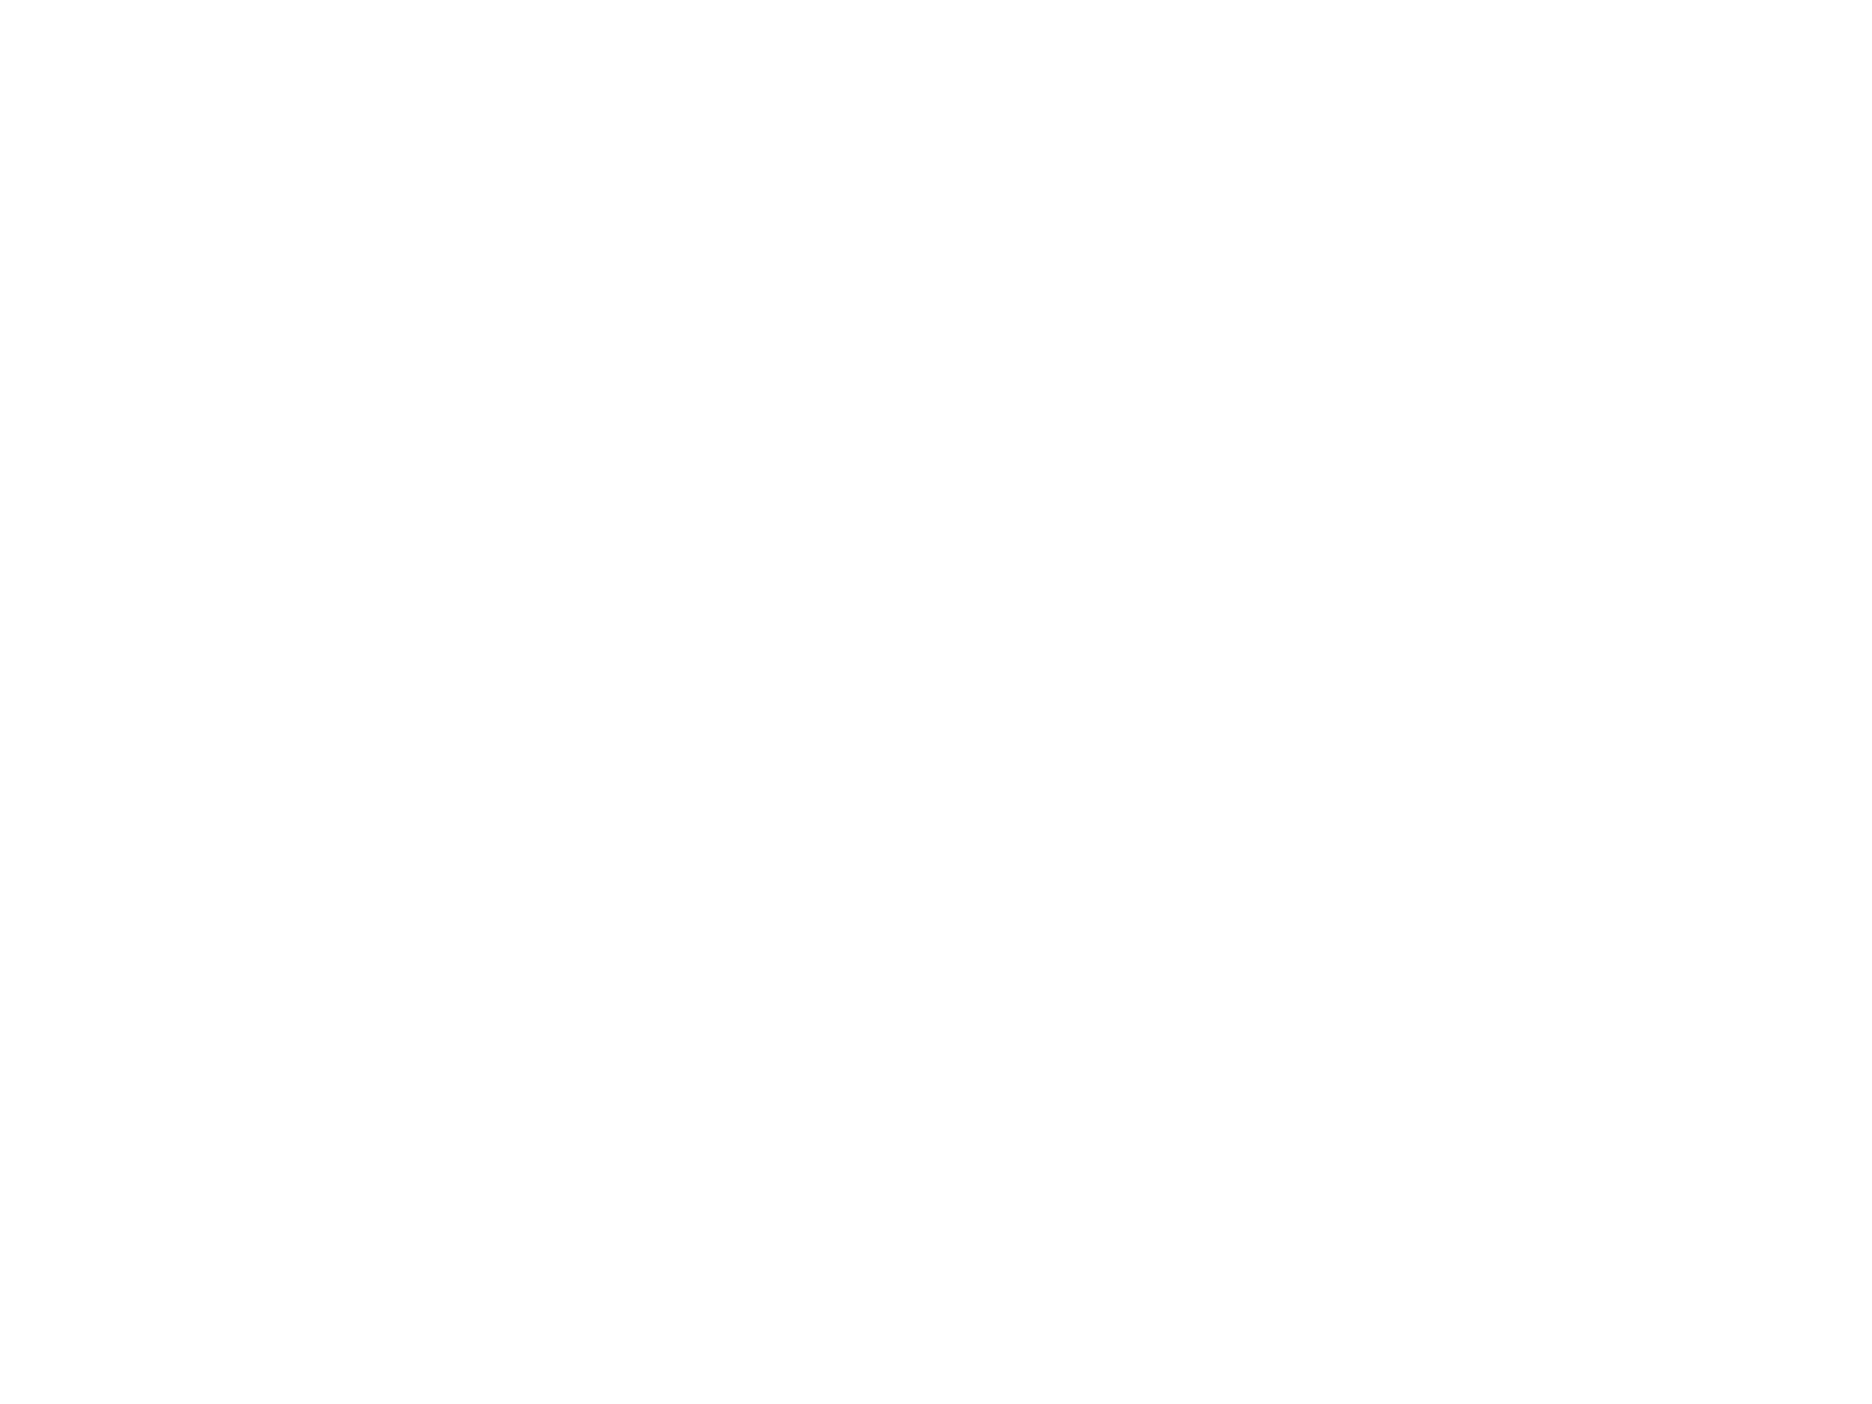
\includegraphics[width=\columnwidth]{figures/intro.png}
	\end{center}
	Something's going on...
\end{frame}

\begin{frame}{Preliminaries}
	Let's fix a probability space $W = (W, \F, \P)$.
	Recall that
	\begin{itemize}
		\item $W : \Set$\\
		Space of `outcomes' of a stochastic experiment
		\item $\F : \sigma$-field\\
		Space of `events', i.e. $\sigma$-algebra of subsets of $W$
		\item $\P : \F \to [0,1]$\\
		'Probability measure', i.e. an assignment of beliefs to events
	\end{itemize}
	\vfill
	\begin{center}
		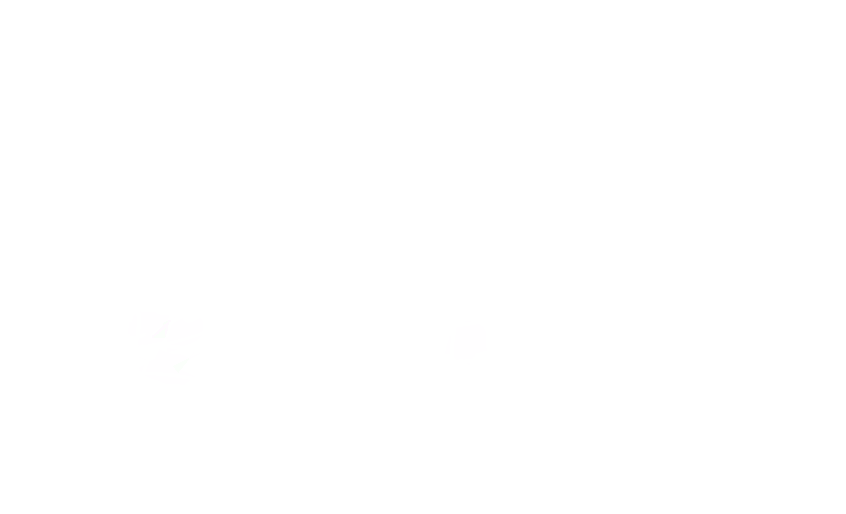
\includegraphics[width=.45\columnwidth]{figures/proba-space.png}
	\end{center}
\end{frame}

\begin{frame}{Preliminaries}
	We call
	\begin{equation*}
		\ker \P = \{A \in \F \suchthat \P(A) = 0 \}
	\end{equation*}
	the $\sigma$-ideal of null sets.

	\vfill
	Let $V = (V, \G, \Q)$.
	\begin{center}
		\text{\underline{measurable maps}}\\
		$\Msbl(W, V) = \{ f : W \to V \suchthat f^{-1}\G \subseteq \F\}$\\[2ex]

		\text{\underline{null-reflecting maps}}\\
		$\Msbl_0(W, V) = \{ f \in \Msbl(W, V) \suchthat f^{-1}\ker\Q \subseteq \ker \P\}$
	\end{center}
\end{frame}

\begin{frame}{Preliminaries}
	\begin{definition}
		An $E$-valued \textbf{stochastic process} on $W$ is a collection of measurable maps
		\begin{equation*}
			X_t : W \to E, \qquad t \in I
		\end{equation*}
		where $I$ is a poset of \textbf{time}s and $E$ is a measurable space of \textbf{values}.
	\end{definition}

	\begin{example}
		Toss a coin and bet $1\$$ on heads: $W = \{H,T\}^\N$, $E = \Z$, $I = \N$,
		\begin{equation*}
			X_n(\omega) = \sum_{i=0}^n (\delta^{\omega_i}_H(\omega) - \delta^{\omega_i}_T(\omega))
		\end{equation*}
	\end{example}
	\vspace{-3ex}
	\begin{example}
		Prices of a market form a stochastic process $M_t$. The value of your portfolio is a certain function $X_t = f(M_t)$.
	\end{example}
\end{frame}

\begin{frame}{Preliminaries}
	A central concept in stochastic calculus is that of filtration:
	\begin{definition}
		A \textbf{filtration} on $W$ is a sequence of $\sigma$-fields $\{\F_t\}_{t \in I}$ such that $\F_t \subseteq \F_s$ when $t \leq s$. One sets $\F_\infty := \F$.
	\end{definition}

	\vfill
	It gives a `\gold{\bfseries causal structure}' to the observed events.

	\vfill
	\begin{definition}
		An \textbf{adapted process} is a process $\{X_t\}_{t \in I}$ such that
		\begin{center}
			for each $t \in I$, \quad $X_t$ is $\F_t$-measurable.
		\end{center}
	\end{definition}
	i.e. the value of $X$ at $t$ only depends on info available until that point.
\end{frame}

\begin{frame}{Preliminaries}
	\textbf{It\^o calculus}: a popular way to do stochastic calculus
	\begin{enumerate}
		\item We can \textbf{integrate} wrt stochastic processes:
		\begin{equation*}
			\int_0^t X_t \, \de B_t = \lim_n\; {\textstyle \sum_i}\, X^{(n)}_{t_i} \, (B_{t_{i+1}} - B_{t_i})
		\end{equation*}
		\item We can discuss \textbf{differential problems}:
		\begin{equation*}
			\de X_t = \sigma_t X_t \de B_t + \mu_t X_t \de t
		\end{equation*}
	\end{enumerate}

	\vfill
	\gold{Here $B_t$ is a \textbf{Brownian motion} $\rightsquigarrow$ archetypal diffusion process}

	\vfill
	It's not exactly like elementary calculus though, e.g.
	\begin{equation*}
		\de f(B_t) = f'(B_t)\,\de B_t + \frac12 f''(B_t) \de t
	\end{equation*}
	because $B_t$ has 'unbounded variation'
\end{frame}

\begin{frame}{Idea}
	Original goal:
	\vfill
	\vspace{-3ex}
	\begin{center}
	\Huge
		$\Underset{\text{\LARGE\color{colorgold}topos}}{\text{stochastic}}
		\
		\Overset{\text{\LARGE\color{colorgold}`elementary'}}{\text{calculus}}$
	\end{center}
	\vfill
	It turned out to be much harder than I thought\\
	and probably not that simple
	\begin{center}
		\textit{...still, plenty of interesting stuff along the way!}
	\end{center}

	\vfill
	\gold{\textbf{Warning}: work still in progress!}
\end{frame}
